\chapter{Entropy and Cross Entropy}
\section{Codes}
Let me tell you about my imaginary friend, Bob. Bob really likes animals. He constantly talks about animals.
In fact, he only ever says four words: "dog", "cat", "fish" and "bird".

A couple weeks ago, despite being a figment of my imagination, Bob moved to Australia.
Further, he decided he only wanted to communicate in binary. All my (imaginary) messages from Bob look like this: 100110$\ldots$.
To communicate, Bob and I have to establish a code, a way of mapping words into sequences of bits.

\begin{figure}[htbp]
  \centering
  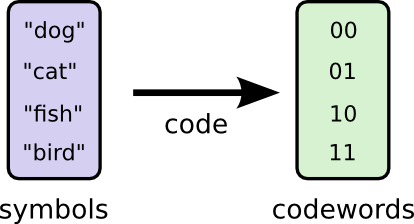
\includegraphics[scale = 0.8]{code-2bit}\\
  \caption{Symbol to codewords}\label{fig.entropy.word2code}
\end{figure}

To send a message, Bob replaces each symbol (word) with the corresponding codeword, and then concatenates them together to form the encoded string.

\begin{figure}[htbp]
  \centering
  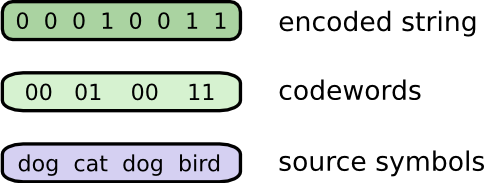
\includegraphics[scale = 0.8]{encode-2bit}\\
  \caption{code to words}\label{fig.entropy.code2word}
\end{figure}

\section{Variable-Length Codes}
Unfortunately, communication services in imaginary-Australia are expensive. 
Bob and I decided we should investigate whether there was some way we could make our average message length shorter.

As it turns out Bob doesn't say all words equally often. Bob really likes dogs. Here's a graph of his word frequency:

\begin{figure}[htbp]
  \centering
  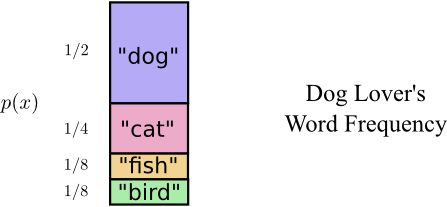
\includegraphics[scale = 0.9]{DogWordFreq}\\
  \caption{DogWordFreq}\label{fig.entropy.DogWordFreq}
\end{figure}

That seems promising. Our old code uses codewords that are 2 bits long, regardless of how common they are.

There’s a nice way to visualize this. In the following diagram, we use the vertical axis to visualize the probability of each word, $p(x)$,
and the horizontal axis to visualize the length of the corresponding codeword, $L(x)$.
Notice that the area is the average length of a codeword we send – in this case 2 bits.

\begin{figure}[htbp]
  \centering
  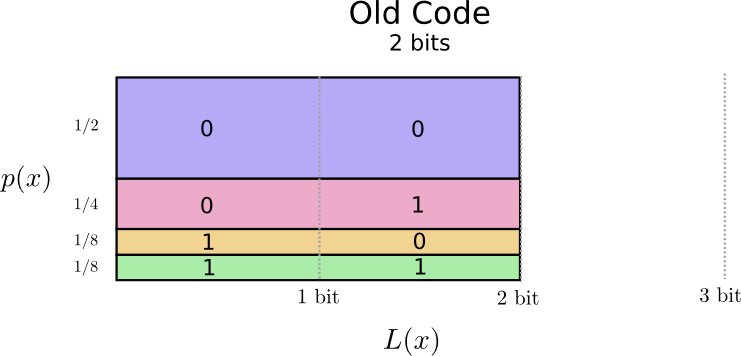
\includegraphics[scale = 0.8]{OldCode}\\
  \caption{OldCode}\label{fig.entropy.OldCode}
\end{figure}

Perhaps we could be very clever and make a variable-length code where codewords for common words are made especially short.
The challenge is that there's competition between codewords – making some shorter forces us to make others longer.
To minimize the message length, we'd ideally like all codewords to be short, but we especially want the commonly used ones to be.
So the resulting code has shorter codewords for common words (like "dog") and longer codewords for less common words (like "bird").

\begin{figure}[htbp]
  \centering
  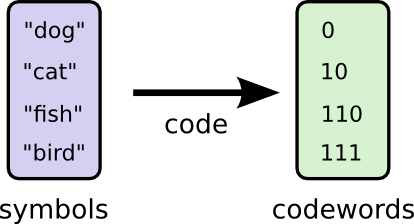
\includegraphics[scale = 0.8]{code}\\
  \caption{code}\label{fig.entropy.code}
\end{figure}

\begin{figure}[htbp]
  \centering
  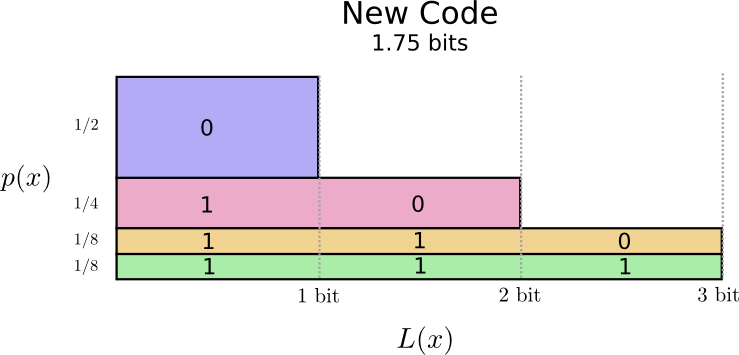
\includegraphics[scale = 0.8]{NewCode}\\
  \caption{NewCode}\label{fig.entropy.NewCode}
\end{figure}
$$ 1 \times 1/2 + 2 \times 1/4 + 3 \times 1/8 + 3 \times 1/8 = 1.75$$

It turns out that this code is the best possible code.
There is no code which, for this distribution, will give us an average codeword length of less than 1.75 bits.

We call this fundamental limit the entropy of the distribution.

\section{The Space of Codewords}
One useful way to think about this is that every codeword requires a sacrifice from the space of possible codewords.
If we take the codeword 01, we lose the ability to use any codewords it's a prefix of.
We can't use 010 or 011010110 anymore because of ambiguity – they're lost to us.

Since a quarter of all codewords start with 01, we've sacrificed a quarter of all possible codewords.
That's the price we pay in exchange for having one codeword that's only 2 bits long!
In turn this sacrifice means that all the other codewords need to be a bit longer.
There's always this sort of trade off between the lengths of the different codewords.
A short codeword requires you to sacrifice more of the space of possible codewords, preventing other codewords from being short.
What we need to figure out is what the right trade off to make is!

You can think of this like having a limited budget to spend on getting short codewords.
We pay for one codeword by sacrificing a fraction of possible codewords.

The cost of buying a codeword of length 0 is 1, all possible codewords – if you want to have a codeword of length 0, you can't have any other codeword.
The cost of a codeword of length 1, like "0", is 1/2 because half of possible codewords start with "0".
The cost of a codeword of length 2, like "01", is 1/4 because a quarter of all possible codewords start with "01".
In general, the cost of codewords decreases exponentially with the length of the codeword.

\section{Calculating Entropy}
Recall that the cost of a message of length $L$ is $1/2^L$.
$$cost = 1/2^L \Rightarrow L = \log_2{1/cost}$$

Since we spend $p(x)$ on a codeword for $x$, the length is $\log_2{1/p(x)}$. Those are the best choices of lengths.

Earlier, we discussed how there is a fundamental limit to how short one can get the average message to communicate events
from a particular probability distribution, $p$.
This limit, the average message length using the best possible code, is called the entropy of $p$, $H(p)$.
Now that we know the optimal lengths of the codewords, we can actually calculate it!
$$H(p) = \sum_x p(x)\log_2\left(\frac{1}{p(x)}\right)$$

No matter what I do, on average I need to send at least that number of bits if I want to communicate which event occurred.

The average amount of information needed to communicate something has clear implications for compression.
But are there other reasons we should care about it? Yes! It describes how uncertain I am and gives a way to quantify information.

If I knew for sure what was going to happen, I wouldn't have to send a message at all!
If there's two things that could happen with $50\%$ probability, I only need to send 1 bit.
But if there's 64 different things that could happen with equal probability, I'd have to send 6($\log_2{64}$) bits.
The more concentrated the probability, the more I can craft a clever code with short average messages.
The more diffuse the probability, the longer my messages have to be.

The more uncertain the outcome, the more I learn, on average, when I find out what happened.

\section{Cross-Entropy}
Shortly before his move to Australia, Bob married Alice, another figment of my imagination.
To the surprise of myself, and also the other characters in my head, Alice was not a dog lover. She was a cat lover.
Despite this, the two of them were able to find common ground in their shared obsession with animals and very limited vocabulary size.

\begin{figure}[htbp]
  \centering
  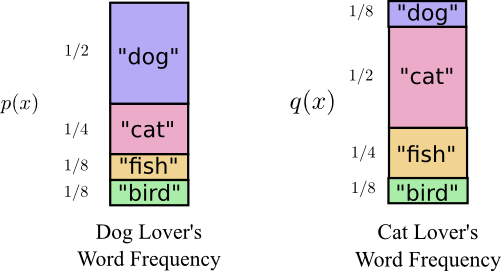
\includegraphics[scale = 0.8]{DogCatWordFreq}\\
  \caption{DogCatWordFreq}\label{fig.entropy.DogCatWordFreq}
\end{figure}

The two of them say the same words, just at different frequencies. Bob talks about dogs all the time, Alice talks about cats all the time.

Initially, Alice sent me messages using Bob's code. Unfortunately, her messages were longer than they needed to be.
Bob's code was optimized to his probability distribution. Alice has a different probability distribution, and the code is suboptimal for it.
While the average length of a codeword when Bob uses his own code is 1.75 bits, when Alice uses his code it's 2.25.
It would be worse if the two weren't so similar!

This length – the average length of communicating an event from one distribution with the optimal code for another distribution – 
is called the cross-entropy.
Formally, we can define cross-entropy as:
$$H_p(q) = \sum_x q(x)\log_2\left(\frac{1}{p(x)}\right)$$
In this case, it's the cross-entropy of Alice the cat-lovers word frequency with respect to the Bob the dog-lovers word frequency.

To keep the cost of our communications down, I asked Alice to use her own code. To my relief, this pushed down her average message length.
But it introduced a new problem: sometimes Bob would accidentally use Alice's code.
Surprisingly, it's worse for Bob to accidentally use Alice's code than for Alice to use his!

So, now we have four possibilities:
\begin{itemize}
\item So, Bob using his own code ($H(p)=1.75$ bits)
\item So, Alice using Bob's code ($Hp(q)=2.25$ bits)
\item So, Alice using her own code ($H(q)=1.75$ bits)
\item So, Bob using Alice's code ($Hq(p)=2.375$ bits)
\end{itemize}

This isn't necessarily as intuitive as one might think. For example, we can see that $H_p(q) \neq H_q(p)$.
Is there some way we can see how these four values relate to each other?

In the following diagram, each subplot represents one of these 4 possibilities.
Each subplot visualizes average message length the same way our previous diagrams did.
They are organized in a square, so that if the messages are coming from the same distribution the plots are beside each other,
and if they use the same codes they are on top of each other. This allows you to kind of visually slide the distributions and codes together.

\begin{figure}[htbp]
  \centering
  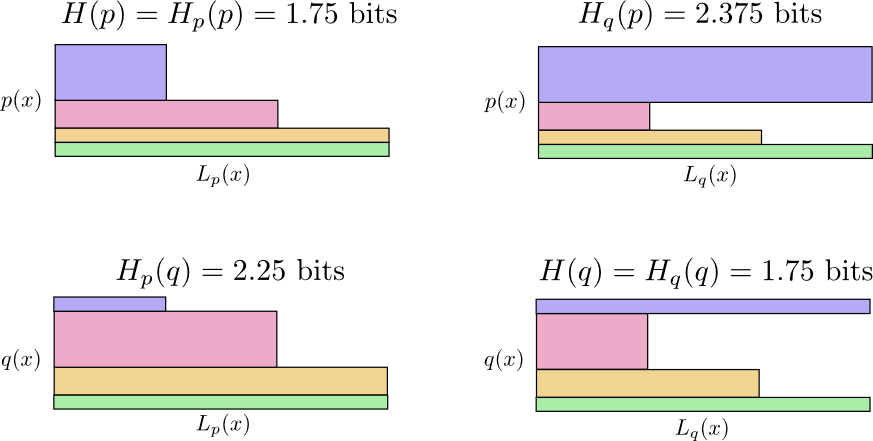
\includegraphics[scale = 0.8]{CrossEntropyCompare}\\
  \caption{CrossEntropyCompare}\label{fig.entropy.CrossEntropyCompare}
\end{figure}

Can you see why $H_p(q) \neq H_q(p)$?
$H_q(p)$ is large because there is an event (blue) which is very common under $p$ but gets a long code because it is very uncommon under $q$.
On the other hand, common events under $q$ are less common under $p$, but the difference is less drastic, so $H_p(q)$ isn't as high.

Cross-entropy isn't symmetric.

So, why should you care about cross-entropy? Well, \textbf{cross-entropy gives us a way to express how different two probability distributions are.}
The more different the distributions p and q are, the more the cross-entropy of p with respect to q will be bigger than the entropy of p.

Similarly, the more different p is from q, the more the cross-entropy of q with respect to p will be bigger than the entropy of q.

The really interesting thing is the difference between the entropy and the cross-entropy.
That difference is how much longer our messages are because we used a code optimized for a different distribution.
If the distributions are the same, this difference will be zero. As the difference grows, it will get bigger.

We call this difference the Kullback–Leibler divergence, or just the KL divergence. The KL divergence of p with respect to q, Dq(p), is defined:
$$D_q(p) = H_q(p) - H(p)$$

The really neat thing about KL divergence is that it's like a distance between two distributions.
It measures how different they are! (If you take that idea seriously, you end up with information geometry.)

Cross-Entropy and KL divergence are incredibly useful in machine learning. Often, we want one distribution to be close to another.
For example, we might want a predicted distribution to be close to the ground truth.
KL divergence gives us a natural way to do this, and so it shows up everywhere.

\section{Entropy and Multiple Variables}
We call this the joint entropy of X and Y, defined:
$$H(X,Y) = \sum_{x,y} p(x,y) \log_2\left(\frac{1}{p(x,y)}\right)$$

We call this the conditional entropy.
$$
H(X|Y)
= \sum_y p(y) \sum_x p(x|y) \log_2\left(\frac{1}{p(x|y)}\right)
= \sum_{x,y} p(x,y) \log_2\left(\frac{1}{p(x|y)}\right)
$$


\section*{Ref}
\href{http://colah.github.io/posts/2015-09-Visual-Information/}{Visual Information Theory}

